% Location, location, location: does a tabular foundation model need spatial features?
% arXiv-ready (pdflatex). Build:
%   pdflatex "Location, location, location - does a tabular foundation model need spatial features"
%   bibtex   "Location, location, location - does a tabular foundation model need spatial features"
%   pdflatex (twice more)
% Every number in this manuscript is read from the versioned results in ../results/ and
% ../data/ and verified by paper/check_numbers.py.
\documentclass[11pt,a4paper]{article}
\usepackage[margin=2.5cm]{geometry}
\usepackage[utf8]{inputenc}
\usepackage[T1]{fontenc}
\IfFileExists{lmodern.sty}{\usepackage{lmodern}}{}
\usepackage[expansion=false]{microtype}
\usepackage{amsmath,amssymb}
\usepackage{booktabs}
\usepackage{graphicx}
\usepackage{caption}
\usepackage{subcaption}
\usepackage{xcolor}
\usepackage{url}
\usepackage[hidelinks]{hyperref}
\usepackage[numbers,sort&compress]{natbib}
\graphicspath{{figures/}}
\captionsetup{font=small,labelfont=bf}
\setlength{\bibsep}{1.6pt plus 0.3ex}
\setlength{\textfloatsep}{9pt plus 2pt minus 4pt}
\setlength{\floatsep}{7pt plus 2pt minus 3pt}
\setlength{\abovecaptionskip}{5pt}
\setlength{\emergencystretch}{1.5em}
\newcommand{\Rsqm}{R\$/m\textsuperscript{2}}

\title{Location, location, location: does a tabular foundation model need spatial features?\\
\large TabPFN-3.5 against spatial econometrics and gradient boosting on 130{,}000 declared
transaction prices in São Paulo}

\author{Agnaldo Calvi Benvenho\thanks{IBAPE Nacional (Brazilian Institute of Engineering
Appraisals and Expert Examinations) and Universidade Presbiteriana Mackenzie, São Paulo, Brazil.
\texttt{agnaldo.benvenho@gmail.com}. Code and data:
\url{https://github.com/abenvenho/tabpfn-itbi-sp}.}}
\date{October 2026}

\begin{document}
\maketitle

\begin{abstract}
Mass appraisal models encode the dependence of property prices on location explicitly, through
spatial weights matrices, spatial lags, geographically weighted local models or engineered
neighbourhood features. We ask whether a tabular foundation model can do without them.
TabPFN-3.5 receives the property attributes and the geographic coordinates as two ordinary numeric
columns, with no spatial modelling of any kind, and is compared with an OLS hedonic model, a
spatial autoregressive lag model (SAR, GM estimation), XGBoost with a $k$-nearest-neighbour
spatial lag, rotated coordinates and nested tuning, and a geographically weighted XGBoost. The
data are 82{,}187 declared transaction prices from the São Paulo real-estate transfer tax (ITBI)
in 2025 and 47{,}810 in the first seven months of 2026, for apartments, houses and commercial
units. The evaluation has two legs: leave-one-block-out cross-validation over ten spatial blocks,
and an out-of-time test that fits on 2025 and predicts 2026. Refutation criteria were fixed in
advance: worse pooled error, losses in most blocks under paired tests, or more residual spatial
autocorrelation (Moran's~$I$) than the explicitly spatial baselines. Out of time, the plain-table
model beats all three spatial specialists in at least 9 of 10 blocks (RMSE $0.265$ in log unit
price against $0.283$--$0.326$; MAPE $19.5\%$ against $20.9$--$25.0\%$) and leaves the least
residual autocorrelation of the models compared ($I = 0.092$); with the raw postal code in place
of the coordinates --- one text column, no geometry --- every one of those verdicts holds. Across
unseen blocks it ties both XGBoost variants on error and beats SAR, but leaves more spatial
structure in its residuals ($I = 0.348$ against $0.309$--$0.326$), a partial refutation, on the
record. Permutation SHAP shows the two coordinates as the model's strongest inputs; the
postal-code result shows that what they carry, inside an observed market, is location as an
identifier rather than geometry, and that only coordinates extrapolate to districts without sales.
For mass appraisal inside a market with a sales history, a foundation model given the raw table is
the strongest predictor in this comparison, with one fit of fifteen seconds and no spatial
engineering.
\end{abstract}

\noindent\textbf{Keywords:} mass appraisal; tabular foundation models; TabPFN; spatial
autoregression; spatial cross-validation; hedonic prices; São Paulo.

\section{Introduction}
\label{sec:intro}

Mass appraisal at city scale rests on the hedonic view of the property market
\citep{rosen1974}: the price of a heterogeneous good is a function of its attributes, and
location is the attribute that dominates the others --- near things are more related than distant
things \citep{tobler1970}. Prices of neighbouring properties are therefore not independent
observations, which breaks the assumption behind the ordinary least squares regression that
appraisal practice relies on \citep{anselin1988}. The established answers model the dependence
explicitly: a spatial weights matrix and an autoregressive term in spatial econometrics
\citep{anselin1988,lesage2009}, local models re-fitted across the map in geographically weighted
regression \citep{fotheringham2002} and its tree-based descendants \citep{grekousis2025}, or
neighbourhood features hand-fed to a gradient-boosting learner. All of it works, and all of it is
engineering that has to be redone for every city and every dataset: a weights matrix to build, a
bandwidth to tune, a lag to recompute inside every training fold.

Tabular foundation models offer a different bargain. TabPFN is a transformer
\citep{vaswani2017} pre-trained on millions of synthetic tabular tasks; at use time it performs
in-context learning, taking the whole training table as its prompt and predicting the test rows
in one forward pass, with no gradient steps and no tuning
\citep{hollmann2023tabpfn,hollmann2025nature}. The third generation extended the approach to
large tables and regression \citep{priorlabs2026tabpfn3}, and version 3.5 reads
high-cardinality categorical and free-text columns natively \citep{priorlabs2026tabpfn35}.
Whether such a model, handed latitude and longitude as two plain numeric columns, learns the
spatial dependence that the specialists encode by construction is an open empirical question ---
and a practical one, because if it does, the spatial machinery above becomes optional for a large
class of valuation problems.

The question has a concrete origin. In a comparative study on 5{,}005 apartment listings in Belo
Horizonte, Brazil, TabPFN v3 with raw coordinates outperformed OLS, SAR, SEM and a
semiparametric spatial lag model under spatial block cross-validation \citep{benvenho2026cead}.
That result invited a harder test, and this paper is that test: declared transaction prices
instead of listings, three property types instead of one, 82{,}187 training rows instead of
5{,}005, a one-year-ahead leg on top of the spatial block cross-validation, a residual
autocorrelation criterion that can refute the claim even where the error cannot, and a stronger
set of spatial opponents. The framing is falsificationist: the hypothesis is stated before the
runs, with the criteria that would refute it, and the comparison is deliberately asymmetric
\emph{against} it --- the baselines keep every spatial advantage, the foundation model gets the
plain table.

The hypothesis is stated so that it can fail:

\begin{quote}
A tabular foundation model that receives only the property attributes and the coordinates as two
plain numeric columns --- no spatial weights matrix, no spatial lag, no engineered neighbourhood
features --- predicts spatially correlated prices as well as, or better than, specialised models
that encode spatial dependence explicitly.
\end{quote}

It is refuted if any of the following holds under a shared protocol: worse pooled RMSE or MAPE;
losses in most spatial blocks under paired tests; or more spatial autocorrelation left in its
out-of-fold residuals than the explicitly spatial models leave in theirs.

The paper contributes: (i) a comparison of a tabular foundation model with spatial econometric
and spatially augmented tree baselines --- a geographically weighted XGBoost among them --- on
declared prices at city scale; (ii) a two-leg protocol, spatial block cross-validation plus
out-of-time testing, with pre-registered refutation criteria that include residual spatial
autocorrelation; (iii) ablations that isolate what carries location inside the model, replacing
the coordinates with a raw postal code and adding the free text of the tax form; (iv) a public,
reproducible pipeline over open municipal data; and (v) the finding itself, the partial
refutation included.

\section{Related work}
\label{sec:related}

\paragraph{Spatial hedonic models.} The hedonic framework \citep{rosen1974} combined with
Tobler's first law \citep{tobler1970} leads to the spatial econometric family: the spatial lag
(SAR) and spatial error models, estimated by maximum likelihood or by the generalised-moments
procedure of \citet{kelejian1998}, with the weights matrix as the carrier of the neighbourhood
structure \citep{anselin1988,lesage2009}. Geographically weighted regression drops the global
coefficient vector and re-fits a local model at every calibration location with
distance-decaying weights \citep{fotheringham2002}.

\paragraph{Machine learning with spatial features.} Tree ensembles do not see space unless it is
fed to them. The standard devices are a spatial lag of the target computed from the training
neighbours, coordinate transformations such as oblique or rotated axes \citep{moller2020}, and
distance covariates. Geographical-XGBoost \citep{grekousis2025} transplants the geographically
weighted idea to gradient boosting: one local XGBoost per calibration location, blended with a
global model. Evaluating any of this honestly requires spatial cross-validation, since random
splits let neighbours of a test point sit in its training set
\citep{roberts2017,meyer2022}.

\paragraph{Tabular foundation models, and space inside them.} TabPFN
\citep{hollmann2023tabpfn,hollmann2025nature} and its third generation
\citep{priorlabs2026tabpfn3,priorlabs2026tabpfn35} replace per-dataset training with in-context
learning over synthetic priors. Two recent lines bring space \emph{to} the model:
TabPFN-GSA modifies the architecture with geospatially aware sparse attention
\citep{deng2026gsa}, and Kriging-prior Regression feeds TabPFN kriging-derived spatial features
\citep{schmidinger2026kpr}. This paper takes the opposite stance: the model as shipped, no
architectural change and no spatial feature, with the dependence left for the in-context learner
to find in two raw columns.

\paragraph{TabPFN in property valuation.} To the author's knowledge, the only published
applications of TabPFN to property valuation are his own, both in Portuguese. On São Paulo
ITBI transaction prices, TabPFN v2 outperformed an FT-Transformer and multiple linear
regression \citep{benvenho2026igel}; on the Belo Horizonte listings, TabPFN v3 outperformed the
linear and non-linear spatial econometric models in the comparison \citep{benvenho2026cead}.
Relative to the latter, the present study changes the target (declared prices instead of
listings), the scope (three property types instead of apartments only), the scale (82{,}187
training rows instead of 5{,}005), the protocol (an out-of-time leg and the residual
autocorrelation criterion are added) and the opponents (a spatially augmented XGBoost and a
geographically weighted XGBoost join the econometric baselines).

\section{Data}
\label{sec:data}

\subsection{Source and cleaning}

The São Paulo City Hall publishes every paid form of the real-estate transfer tax (ITBI,
\emph{Imposto sobre Transmissão de Bens Imóveis}) with the declared transaction price, the
cadastral key (SQL: sector, block, lot) and the physical attributes of the property from the
annual property-tax register (IPTU): built and lot area, use, construction standard and the corrected
completion year (ACC, \emph{Ano de Constru\c{c}\~ao Corrigido}). The 2025 workbook holds 230{,}525 forms and the January--July 2026 workbook
135{,}655. Coordinates come from the centroids of the fiscal-block polygons of the municipal
cadastre (GeoSampa), so all properties in one city block share a location; distance to the
nearest subway or commuter-rail station is computed from the 203 station points of the same
portal.

Table~\ref{tab:filters} gives the cleaning chain with the record count after each step; the full
report, broken down by property type, is versioned with the data
(\texttt{data/filter\_report.md}). The cleaned bases hold 82{,}187 transactions for 2025
(training) and 47{,}810 for 2026 (test). A stratified sample of 24{,}000 rows of 2025 (12{,}000
apartments, 7{,}000 houses, 5{,}000 commercial units; ``Level~A'') is used wherever the slower
baselines must run.

\begin{table}[t]
\centering\small
\caption{The cleaning chain: records remaining after each step.}
\label{tab:filters}
\footnotesize
\begin{tabular}{clrr}
\toprule
\# & Step & 2025 & 2026 (Jan--Jul) \\
\midrule
0 & Raw base (all paid ITBI forms) & 230{,}525 & 135{,}655 \\
1 & Deed nature contains ``compra e venda'' (sale and purchase) & 207{,}518 & 124{,}289 \\
2 & Transmitted share $= 100\%$ & 108{,}750 & 61{,}304 \\
3 & Cadastral status active & 108{,}420 & 61{,}112 \\
4 & Valid 11-digit SQL key and valid date & 108{,}420 & 61{,}112 \\
5 & Property type kept (apartment / house / commercial) & 90{,}927 & 51{,}919 \\
6 & Built (reference) area $> 0$ & 90{,}927 & 51{,}919 \\
7 & Plausible completion year ($1900 \le \text{ACC} \le$ transaction year) & 90{,}927 & 51{,}918 \\
8 & Deduplication on (key, date, price) & 90{,}673 & 51{,}810 \\
9 & Declared price $\ge$ R\$ 10{,}000 & 89{,}078 & 51{,}202 \\
10 & Price / assessed reference value within $[0.3, 5]$ & 87{,}488 & 50{,}430 \\
11 & Under-declaration: cash deals pegged to the reference value excluded & 84{,}263 & 48{,}879 \\
12 & Tukey fences ($1.5$ IQR) on $\ln(\text{\Rsqm})$, per type, fences from 2025 & 82{,}193 & 47{,}814 \\
13 & Join to fiscal-block centroid (match $99.99\%$) & 82{,}187 & 47{,}810 \\
\bottomrule
\end{tabular}
\end{table}

\subsection{Under-declaration}

The ITBI tax base is $\max(\text{declared price},\ \text{assessed reference value})$, so a buyer
who under-declares has no incentive to declare below the assessed value: under-declared cash
deals bunch exactly at it. The diagnostics found that bunching concentrated in cash purchases,
and the pipeline removes cash transactions declared within $1\%$ of the reference value: 3{,}225
forms in 2025 and 1{,}551 in 2026 (step 11 of Table~\ref{tab:filters}; the residual picture after
the exclusion is in \texttt{data/underdeclaration\_report.md}). Financed deals pass a lender's
underwriting and are kept; Section~\ref{sec:robust} repeats the whole analysis on financed deals
only.

\subsection{Descriptive statistics}

\begin{table}[h]
\centering\small
\caption{The three bases. Unit value $=$ declared price / built area, in \Rsqm.}
\label{tab:data}
\footnotesize
\begin{tabular}{lrrrrrr}
\toprule
Base & Rows & Apartments & Houses & Commercial & Financed & Median unit value \\
\midrule
2025, full (training) & 82{,}187 & 60{,}067 & 15{,}940 & 6{,}180 & 34\% & 4{,}836 \\
2025, Level A (sample) & 24{,}000 & 12{,}000 & 7{,}000 & 5{,}000 & 30\% & 4{,}715 \\
2026, Jan--Jul (test) & 47{,}810 & 35{,}354 & 9{,}429 & 3{,}027 & 42\% & 4{,}970 \\
\bottomrule
\end{tabular}
\end{table}

The response is strongly autocorrelated in space, as urban prices are. Moran's $I$ of the raw
log unit price on the $k$-NN-8 matrix used throughout the paper is $0.430$ on the Level A sample
($z = 141.8$) and $0.506$ on the 2026 base ($z = 235.7$): a property's unit value is close to its
neighbours' far beyond chance, which is exactly the structure the spatial baselines are built to
exploit. Figure~\ref{fig:blocks}(a) shows how the ten spatial blocks tile that structure over the
city. Because coordinates are fiscal-block centroids, location is resolved to the city block rather
than the address --- a conservative choice shared by every model.

\section{Methods}
\label{sec:methods}

\subsection{Target and features}

The target is $y = \ln(\text{price}/\text{built area})$. The information set is the same for
every model: built area, lot area, age, finish grade (IPTU standard level, 0--5), distance to
the nearest station, month index, property type, latitude and longitude. The models differ only
in what they are allowed to do with the last two.

\subsection{Models}

\paragraph{OLS hedonic.} Log-linear in the areas and the distance, quadratic in age, dummies for
type. The coordinates are not covariates: this is the no-location floor of the linear family.

\paragraph{SAR lag.} $y = \rho W y + X\beta + \varepsilon$ with a row-standardised
$k$-nearest-neighbour weights matrix ($k = 8$) built inside each training fold, estimated by the
generalised-moments procedure of \citet{kelejian1998} as implemented in \texttt{spreg}
\citep{rey2010pysal}. A held-out row is predicted by the structural form with the spatial lag
taken over its $k$ nearest \emph{training} rows,
$\hat y_i = \mathbf{x}_i^{\top}\hat\beta + \hat\rho\,\bar y_{N_8(i)}$, where $\bar y_{N_8(i)}$ is
the mean observed target of those neighbours; the reduced form is not available out of sample
without the test rows' own neighbourhood, so nothing from the test set enters the prediction.
Ties in the centroid coordinates are broken by a deterministic sub-metre jitter
($\pm 0.5$~m, seed 42), needed because all transactions of one fiscal block share the exact
centroid.

\paragraph{XGBoost with spatial features.} The hedonic block above plus UTM coordinates, their
projections on axes rotated by $30^{\circ}$, $45^{\circ}$ and $60^{\circ}$ \citep{moller2020},
and a $k$-NN-8 spatial lag of the target computed inside the training fold (leave-one-out for
training rows). Hyper-parameters are tuned by nested Optuna (30 TPE trials, early stopping, up
to 3{,}000 rounds), with an inner leave-one-block-out on the training blocks; the outer test
block never touches tuning \citep{chen2016xgboost,akiba2019optuna}. Three seeds. The search
space and the selected values are in Appendix~\ref{app:hparams}.

\paragraph{Geographically weighted XGBoost.} Geographical-XGBoost \citep{grekousis2025} fits one
local XGBoost per calibration location with bi-square distance weights,
$w = (1 - d^2/h^2)^2$ with $h$ the distance to the $k$-th neighbour, blended with a global model
as $\hat y = \alpha\,\hat y_{\text{local}} + (1 - \alpha)\,\hat y_{\text{global}}$. As packaged,
it calibrates one local model, with its own grid search, at every training row over a dense
distance matrix, which a feasibility pilot found impracticable at this scale
(Appendix~\ref{app:gxgb}). The implementation here keeps the estimator and calibrates the local
models at 1{,}000 regression points --- the $K$-means centres of the training coordinates, about
one per 1.5~km\textsuperscript{2} of the city --- as geographically weighted regression allows
\citep{fotheringham2002}; a query location is predicted by inverse-distance averaging its three
nearest local models. The local models see the hedonic attributes and no coordinates, so space
enters only through the weighting, as in the original. The bandwidth
$k \in \{50, 100, 200, 400, 800, 1600, 3200\} \times n_{\text{train}}/24{,}000$ and the blend
$\alpha \in \{0, 0.25, 0.5, 0.75, 1\}$ are chosen by an inner block cross-validation inside each
outer fold; the grid was widened downward, from 400 to 50, after the first searches kept
choosing its smallest value, and 50 neighbours is taken as the floor. Three seeds.

\paragraph{TabPFN-3.5, plain table.} The nine raw columns, categorical type declared as such,
through the hosted model (\texttt{tabpfn-client} 0.6.0, model version 3.5). Zero-shot, and a
thinking-mode variant in which the fit explores configurations by internal validation on the
training fold (RMSE objective, medium and high effort). No spatial information of any kind
beyond the two coordinate columns. Fitting on 24{,}000 rows takes about 9~s; on 82{,}187 rows,
15~s. Settings in Appendix~\ref{app:hparams}; the input variants --- the postal code in place of
the coordinates, the free text of the form --- are introduced with their results in
Section~\ref{sec:carriers}.

\subsection{Evaluation protocol}

\paragraph{Leg 1: spatial block cross-validation.} Ten $K$-means blocks on the Level A
coordinates, each held out in turn \citep{roberts2017,meyer2022}. Every fold-internal quantity
(weights matrix, spatial lag, tuning, regression points) is recomputed on the training blocks
only. This asks whether a model can price a part of the city it has never seen --- the harder
test for a model that leans on location.

\paragraph{Leg 2: out-of-time.} One fit on 2025 (Level A, then the full base), predictions for
all 47{,}810 transactions of 2026, one to seven months after the training window. Nothing from
2026 touches fitting or tuning. Same city, so the spatial-lag models get neighbours from the
same streets: the most favourable setting for explicit spatial modelling. Leakage check: no
transaction (key, date, price) appears in both years; $0.6\%$ of 2026 rows share a cadastral key
with Level A.

\paragraph{Metrics and tests.} RMSE, MAE and $R^2$ in log units, MAPE in price units, mean
residual (bias). Residual spatial autocorrelation by Moran's $I$ \citep{moran1950} on a $k$-NN-8
matrix of the test coordinates. Paired comparisons over the ten blocks (for 2026, each
transaction is assigned to the block of its nearest 2025 $K$-means centroid): exact Wilcoxon
signed-rank test on the per-block RMSE and a block bootstrap (2{,}000 resamples of blocks) for
the pooled difference with a 95\% percentile interval. Where a model is stochastic, three seeds
(42, 43, 44) and the per-seed range; a TabPFN run (seed 42) is paired against every seed of a
stochastic opponent.

\section{Results}
\label{sec:results}

\subsection{Leg 1: unseen blocks}

\begin{figure}[t]
\centering
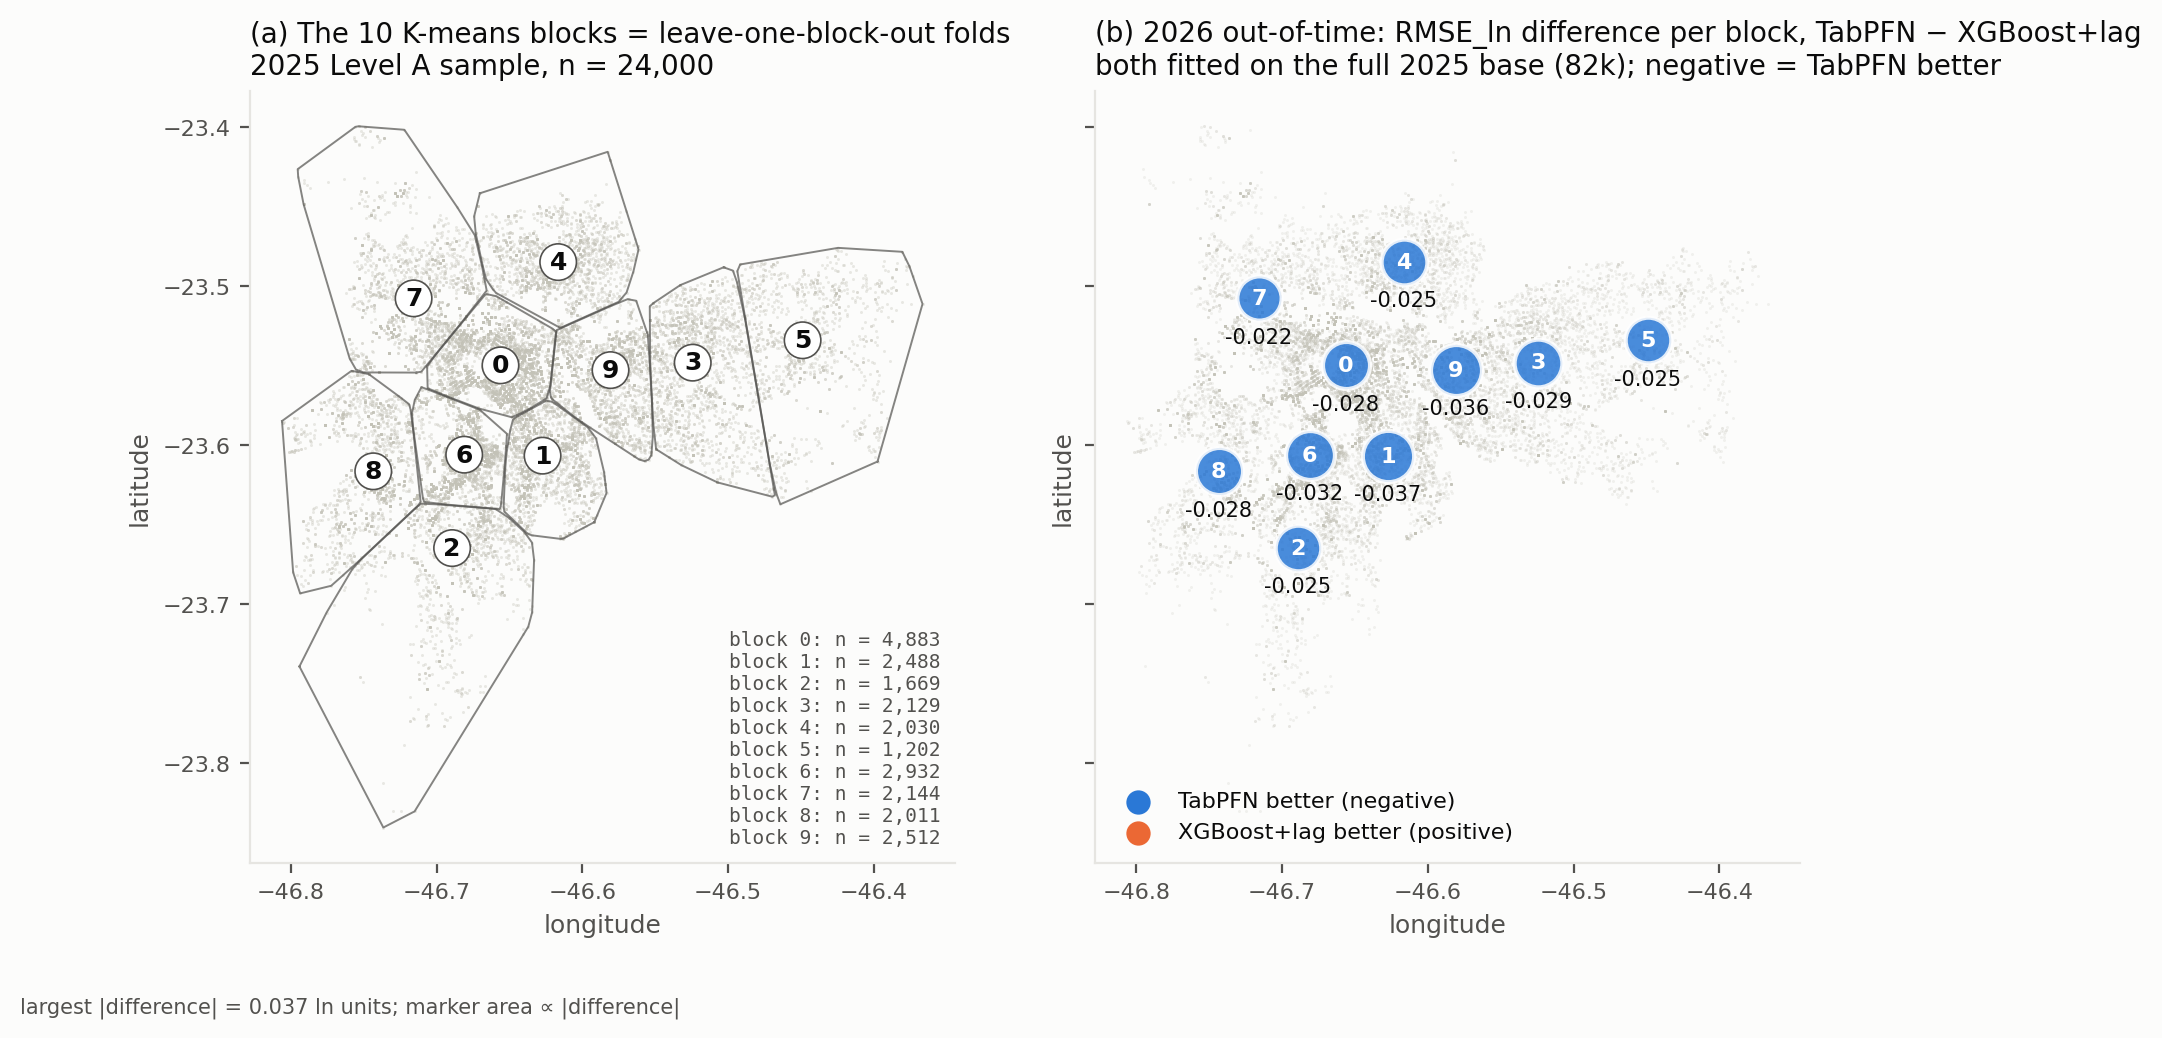
\includegraphics[width=\textwidth]{fig1_blocks_map.png}
\caption{(a) The ten $K$-means blocks of the Level A sample, each held out in turn. (b) Per-block
RMSE difference TabPFN-3.5 $-$ XGBoost+lag on the 2026 test, both fitted on the full 2025 base;
negative in every block.}
\label{fig:blocks}
\end{figure}

\begin{table}[h]
\centering\small
\caption{Leave-one-block-out CV on Level A (24{,}000 rows of 2025). Out-of-fold metrics in log
unit price; Moran's $I$ of the out-of-fold residuals on a $k$-NN-8 matrix. Point values are
seed 42; parenthesised ranges are over three seeds.}
\label{tab:cv}
\footnotesize
\begin{tabular}{lcccc}
\toprule
Model & RMSE & MAPE & $R^2$ & Moran's $I$ \\
\midrule
Median by type (floor) & 0.497 & 42.1\% & $-0.04$ & 0.446 \\
OLS hedonic & 0.470 & 39.4\% & 0.066 & 0.390 \\
SAR lag, GM ($\hat\rho = 0.91$) & 0.448 & 38.4\% & 0.155 & 0.363 \\
XGBoost, rotated coordinates, no lag & 0.397 & 33.3\% & 0.334 & 0.355 \\
XGBoost, rotated coordinates + $k$-NN-8 lag & \textbf{0.385} (0.385--0.387) & 32.3\% & \textbf{0.376} & \textbf{0.309} (0.309--0.318) \\
Geographically weighted XGBoost & 0.410 (0.407--0.410) & 34.5\% & 0.291 & 0.324 (0.319--0.326) \\
TabPFN-3.5, plain table, zero-shot & 0.394 (0.391--0.394) & 32.2\% & 0.346 & 0.348 (0.342--0.348) \\
TabPFN-3.5, plain table, thinking (medium) & 0.389 & \textbf{31.7\%} & 0.362 & 0.342 \\
TabPFN-3.5, plain table, thinking (high) & 0.388 & \textbf{31.7\%} & 0.366 & 0.339 \\
\bottomrule
\end{tabular}
\end{table}

TabPFN-3.5 zero-shot beats the SAR lag model in 8 of 10 blocks ($\Delta$RMSE $= -0.054$, 95\% CI
$[-0.100, -0.014]$, Wilcoxon $p = 0.010$; $\Delta$MAPE $= -6.2$~pp). Against XGBoost with the
explicit lag the difference is a tie: $\Delta$RMSE $= +0.009$ $[-0.018, +0.034]$, 7 blocks won,
one clear loss in the largest block. Against the geographically weighted XGBoost it is also a
tie, leaning TabPFN's way: $\Delta$RMSE $-0.013$ to $-0.016$ across that model's three seeds,
every interval across zero, 6 or 7 blocks won. The two XGBoost variants are not interchangeable:
the geographically weighted one loses to XGBoost+lag by $+0.023$ to $+0.025$ (1 or 2 blocks won,
$p = 0.027$--$0.037$), so the fully spatial global XGBoost is the hardest opponent in this leg.
Thinking mode lowers the zero-shot error by a small margin ($-0.005$ $[-0.008, -0.001]$ against
seed 42, 7 of 10 blocks, though the exact Wilcoxon does not reach significance, $p = 0.105$;
about $-0.002$ against the other seeds) and gives the lowest MAPE in the table;
high effort costs about 13 times more per fold and adds nothing beyond noise.

On the residual criterion the hypothesis is partly refuted in this leg. Moran's $I$ of the
plain-table model ($0.348$) lies below SAR ($0.363$) but above both XGBoost variants: the global
one with the explicit lag ($0.309$) and the geographically weighted one ($0.319$--$0.326$).
Inside XGBoost, the lag alone is worth $\Delta$RMSE $= -0.013$ $[-0.024, -0.004]$ and lowers the
residual $I$ from $0.355$ to $0.309$ --- the measurable value of modelling space explicitly when
the test is a part of the city no model has seen. The refutation is partial and on the record.

Errors are large in absolute terms ($R^2$ of $0.29$--$0.38$ for the non-linear models, against
$0.538$ in the listings
study): declared prices, three property types and centroid coordinates all add noise, and every
model leaves spatial structure behind in this leg.

\subsection{Leg 2: one year ahead}

\begin{table}[h]
\centering\small
\caption{Out-of-time test: fit on 2025, predict the 47{,}810 transactions of 2026. Bias is the
mean residual in log units (positive $=$ under-prediction). Moran's $I$ on a $k$-NN-8 matrix of
the 2026 coordinates. Point values are seed 42; ranges are over three seeds.}
\label{tab:oot}
\scriptsize\setlength{\tabcolsep}{2.6pt}
\begin{tabular}{llccccc}
\toprule
Training base & Model & RMSE & MAPE & $R^2$ & Bias & Moran's $I$ \\
\midrule
Level A (24k) & OLS hedonic & 0.404 & 32.4\% & 0.185 & $+0.033$ & 0.408 \\
 & SAR lag & 0.346 & 27.0\% & 0.401 & $+0.032$ & 0.224 \\
 & XGBoost + lag & 0.288 & 21.8\% & 0.584 & $+0.047$ & 0.138--0.140 \\
 & Geographically weighted XGBoost & 0.313 (0.313--0.314) & 24.0\% & 0.508 & $+0.045$--$+0.048$ & 0.187--0.188 \\
 & TabPFN-3.5, zero-shot & \textbf{0.275} & \textbf{20.4\%} & \textbf{0.622} & $+0.055$ & \textbf{0.122} \\
 & TabPFN-3.5, thinking (medium) & 0.275 & 20.5\% & 0.621 & $+0.055$ & 0.121 \\
\midrule
Full (82k) & OLS hedonic & 0.401 & 32.4\% & 0.194 & $+0.023$ & 0.397 \\
 & SAR lag & 0.326 & 25.0\% & 0.470 & $+0.031$ & 0.134 \\
 & XGBoost + lag & 0.294\textsuperscript{a} & 21.5\%\textsuperscript{a} & 0.568 & $+0.103$\textsuperscript{a} & 0.107\textsuperscript{a} \\
 & Geographically weighted XGBoost & 0.298\textsuperscript{b} & 22.1\% & 0.557 & $+0.065$\textsuperscript{b} & 0.163\textsuperscript{b} \\
 & TabPFN-3.5, zero-shot & \textbf{0.265} & \textbf{19.5\%} & \textbf{0.649} & $+0.058$ & \textbf{0.092} \\
\bottomrule
\end{tabular}\\[2pt]
{\scriptsize \textsuperscript{a}\,seed 42; three seeds: RMSE 0.283--0.294, MAPE 20.9--21.5\%, bias $+0.070$--$+0.103$, $I$ 0.103--0.107.\quad
\textsuperscript{b}\,seed 42; three seeds: RMSE 0.298--0.301, bias $+0.065$--$+0.078$, $I$ 0.163--0.166.}
\end{table}

Paired over the ten 2026 blocks, TabPFN-3.5 zero-shot trained on Level A beats XGBoost with the
explicit lag in 10 of 10 ($\Delta$RMSE $= -0.013$ $[-0.016, -0.011]$, $\Delta$MAPE $= -1.4$~pp,
$p = 0.002$), the geographically weighted XGBoost in 10 of 10 ($-0.038$ to $-0.039$ across its
seeds, every interval within $[-0.049, -0.028]$) and SAR by $-0.071$ $[-0.079, -0.062]$. On the
full base the gap to XGBoost+lag widens to $-0.029$ $[-0.032, -0.026]$ ($\Delta$MAPE
$= -2.0$~pp, again 10 of 10, and by $-0.018$ to $-0.020$ against its two better seeds); against
the geographically weighted XGBoost it is $-0.033$ to $-0.036$ with 9 of 10 blocks ($p = 0.004$;
the one loss is the smallest block, 2{,}425 transactions, by $0.001$--$0.002$), and the
plain-table model has the lowest residual autocorrelation of the five models. Scaling from 24k
to 82k rows improves TabPFN by $-0.010$ $[-0.012, -0.008]$ and SAR by $-0.020$; XGBoost+lag does
not improve ($+0.006$ $[+0.001, +0.011]$ at seed 42) because its trend bias more than doubles,
from $+0.047$ to $+0.103$, and eats the variance gain. The bandwidth of the geographically
weighted model hardly matters here: with 400, 200, 100 or 50 neighbours its 2026 RMSE on
Level A stays between $0.308$ and $0.314$. Errors are flat across blocks ($0.23$--$0.31$) and
across the monthly horizons ($0.26$--$0.28$ over the months with at least 500 transactions): no
subset carries the result. Thinking mode adds nothing in this leg. The hypothesis survives
every criterion, at both scales, against all three spatial specialists.

\begin{figure}[t]
\centering
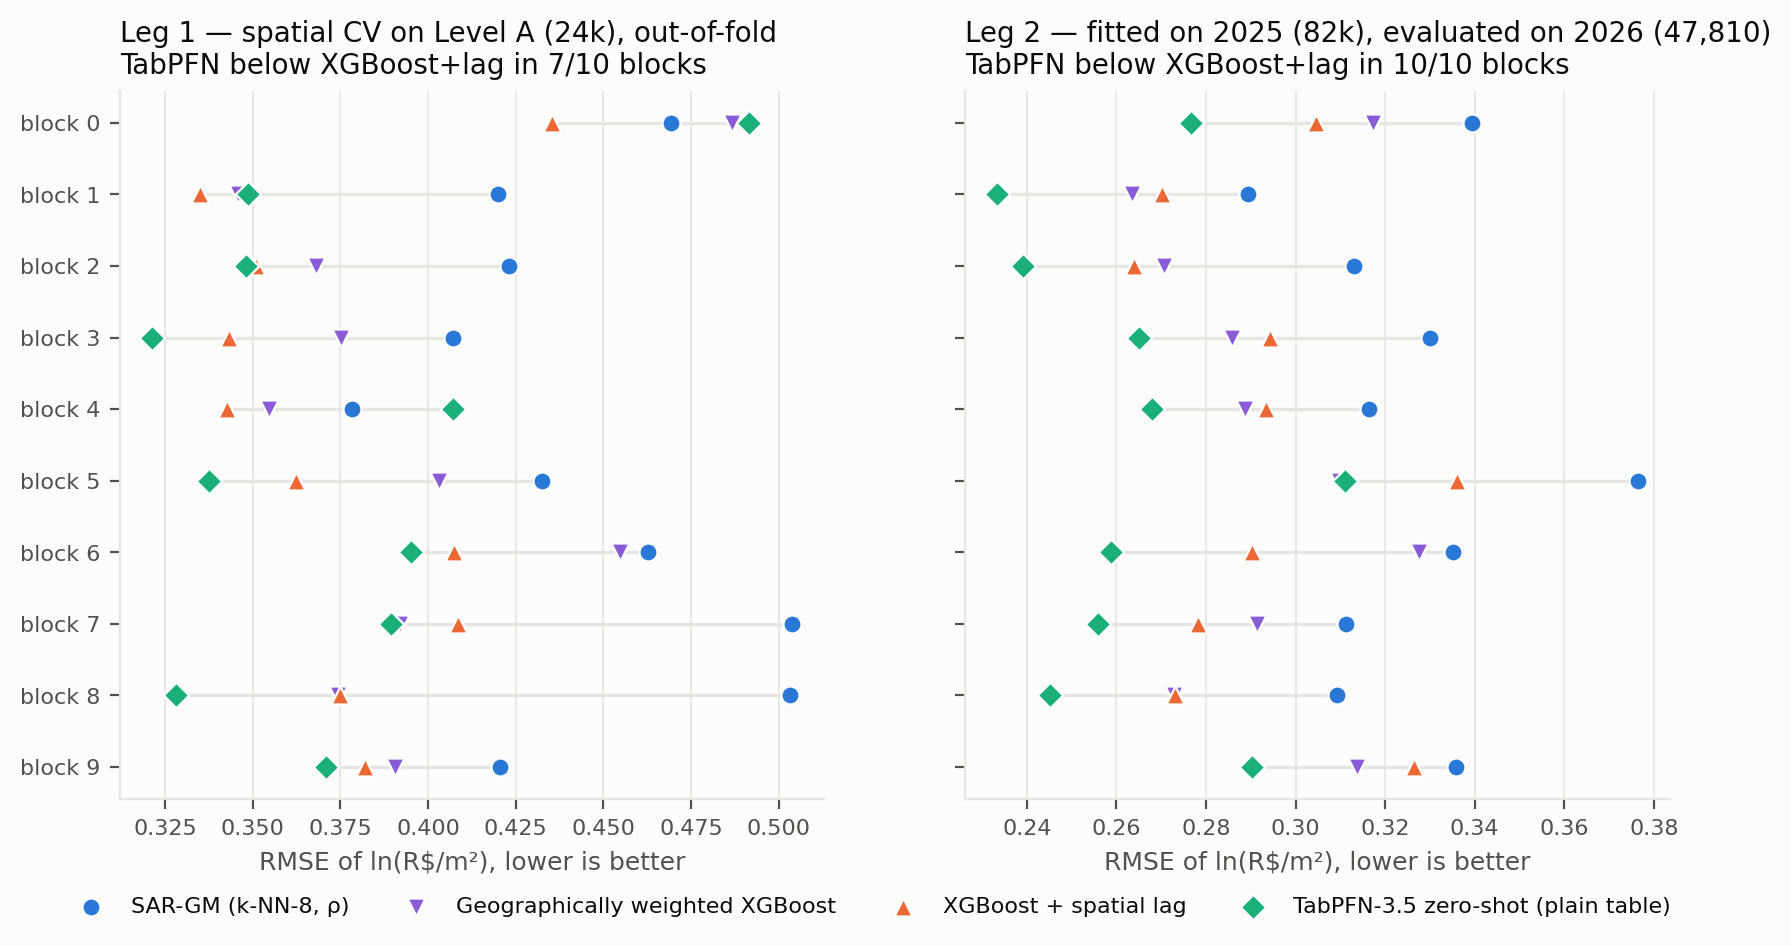
\includegraphics[width=\textwidth]{fig2_per_block_rmse.png}
\caption{RMSE per block. Left panel: leave-one-block-out CV on Level A (leg 1), where TabPFN-3.5
ties XGBoost+lag; right panel: the 2026 out-of-time test with models fitted on the full 2025
base (leg 2), where it is below XGBoost+lag in every block.}
\label{fig:perblock}
\end{figure}

\begin{figure}[t]
\centering
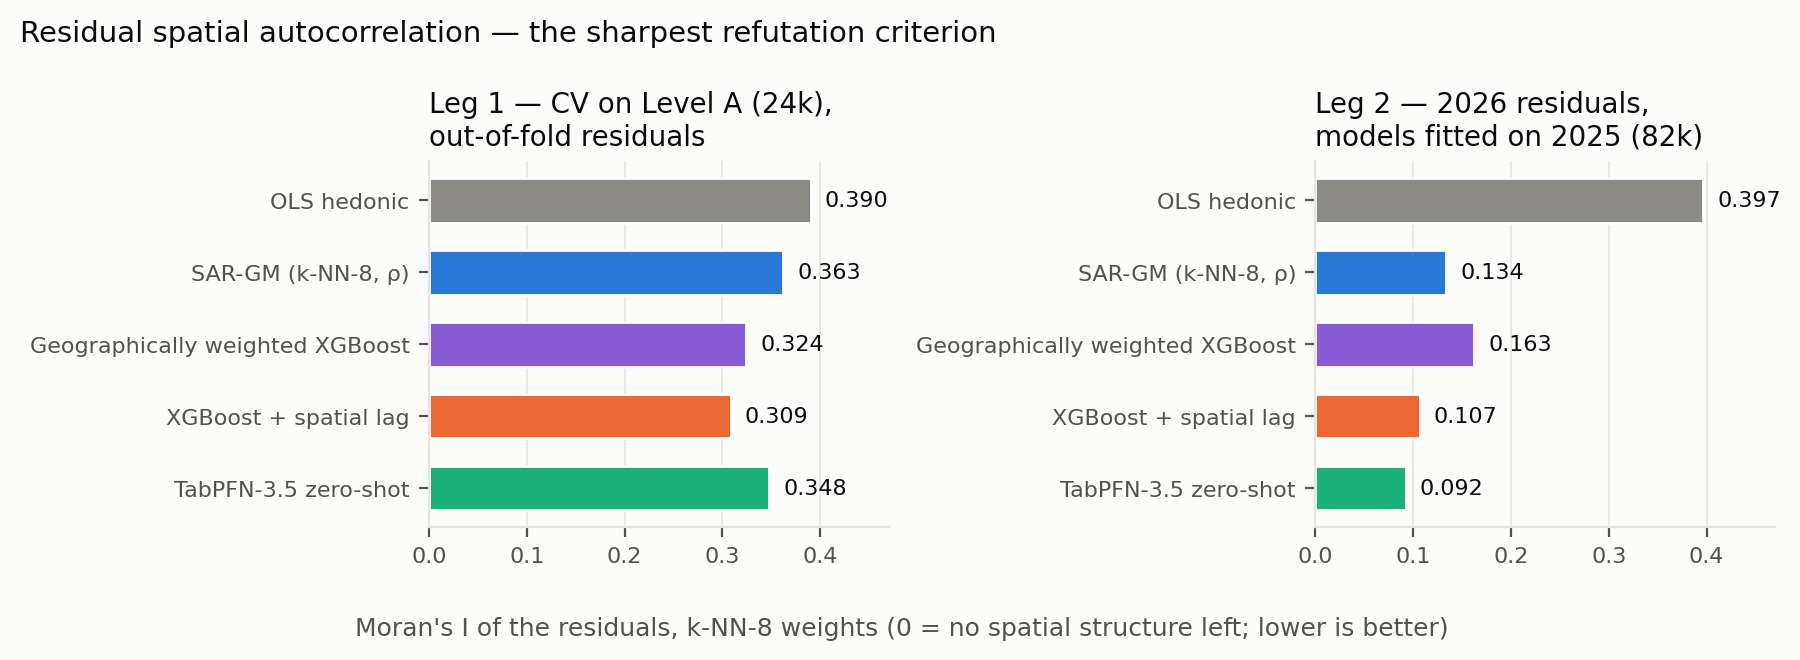
\includegraphics[width=0.9\textwidth]{fig5_moran.png}
\caption{Residual Moran's $I$, the sharpest refutation criterion. Left panel: the block CV
(leg 1), where the plain-table model leaves more spatial structure than either XGBoost --- the
partial refutation; right panel: 2026 (leg 2), where it leaves the least of the five models.}
\label{fig:moran}
\end{figure}

\begin{figure}[t]
\centering
\begin{subfigure}[t]{0.55\textwidth}
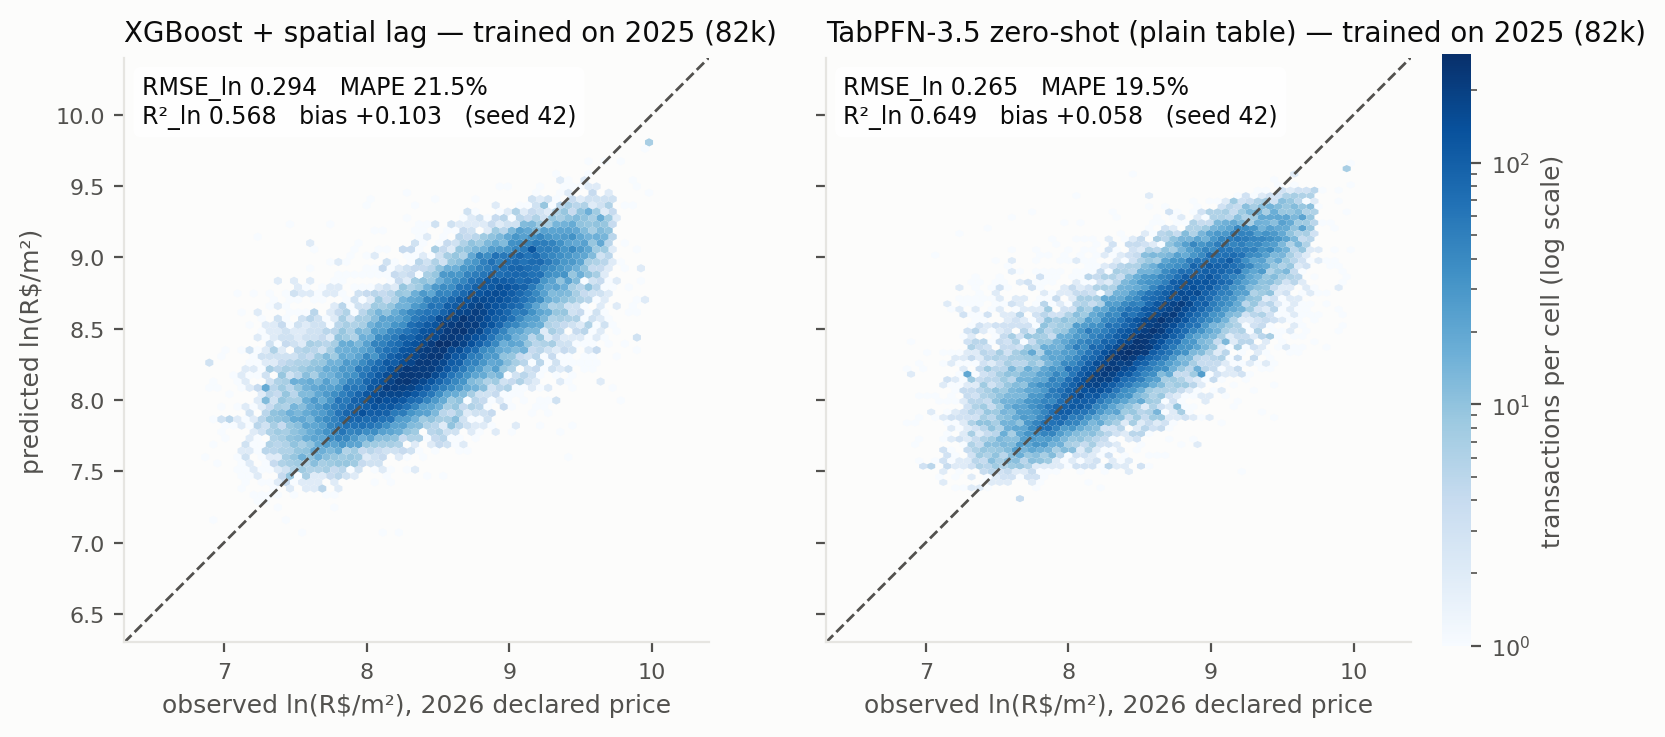
\includegraphics[width=\textwidth]{fig3_pred_vs_obs_2026.png}
\caption{Predicted vs observed, 2026.}
\end{subfigure}\hfill
\begin{subfigure}[t]{0.43\textwidth}
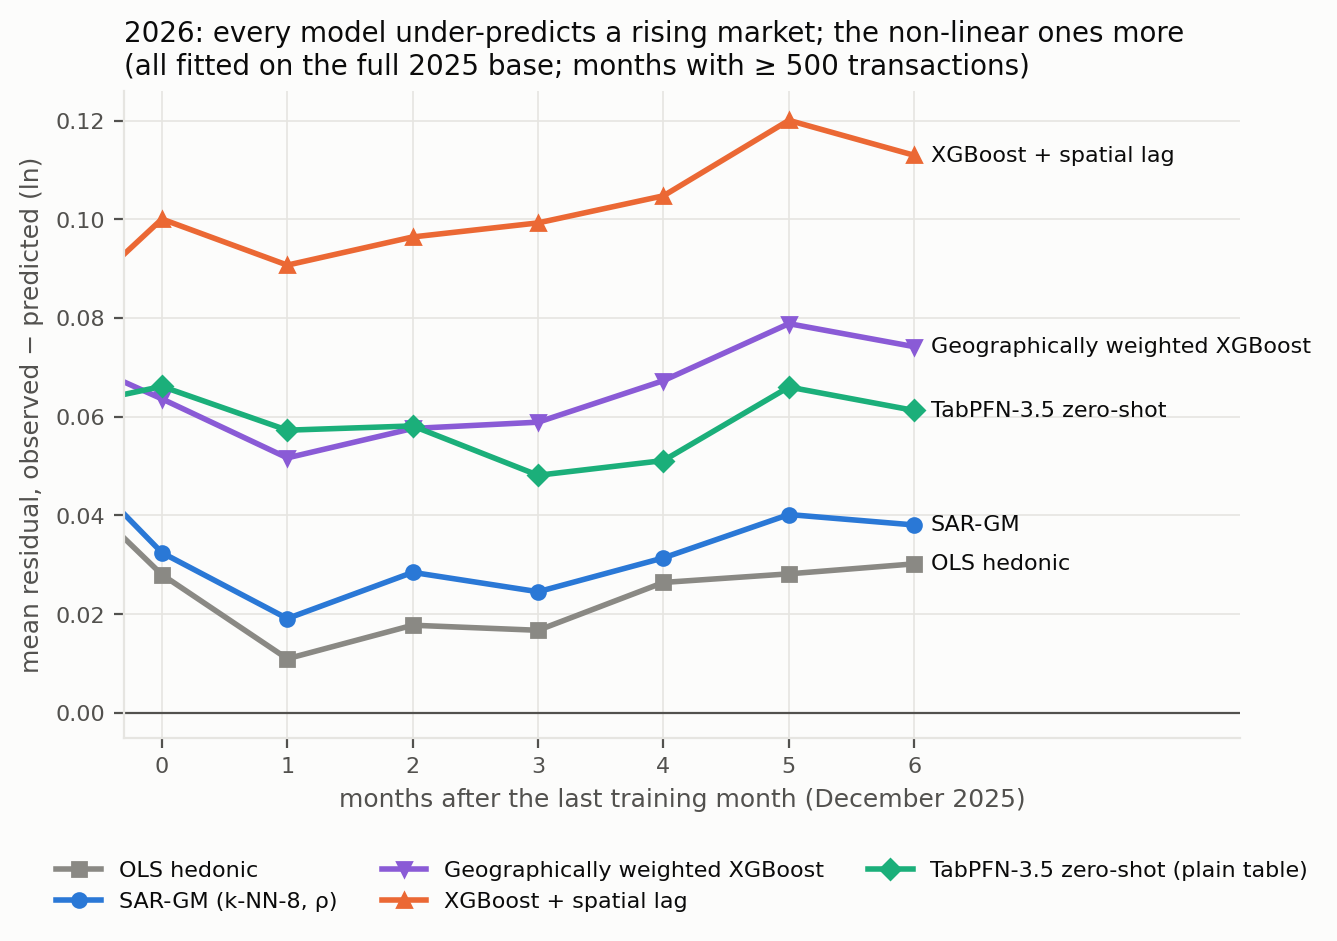
\includegraphics[width=\textwidth]{fig4_months_ahead_bias.png}
\caption{Mean residual by month ahead.}
\end{subfigure}
\caption{The rising market of 2026: every model under-predicts, the non-linear learners more so.}
\label{fig:bias}
\end{figure}

\textbf{The limitation worth stating.} Every model under-predicts 2026, a rising market, and the
non-linear ones more (bias $+0.04$ to $+0.10$ in ln against $+0.02$ to $+0.03$ for OLS and SAR):
trees and TabPFN hold the last observed level of the month index instead of extrapolating a
trend (Figure~\ref{fig:bias}). Appraisal practice would apply a price index; it is reported
here, not corrected.

\subsection{Robustness: financed transactions only}
\label{sec:robust}

Financed transactions carry a bank appraisal and are the cleanest prices in the base. Both legs
were re-run on them alone: 7{,}211 of the 24{,}000 Level A rows for the block CV, the same rows
fitted once and scored on the 20{,}052 financed transactions of 2026.

\begin{table}[h]
\centering\small
\caption{Both legs on financed deals only (seed 42).}
\label{tab:fin}
\footnotesize
\begin{tabular}{lcccccc}
\toprule
Model & CV RMSE & CV MAPE & CV $I$ & 2026 RMSE & 2026 MAPE & 2026 $I$ \\
\midrule
OLS hedonic & 0.354 & 28.5\% & 0.343 & 0.343 & 26.5\% & 0.491 \\
SAR lag & 0.344 & 28.1\% & 0.342 & 0.286 & 22.0\% & 0.297 \\
XGBoost + lag & 0.286 & 23.0\% & 0.327 & 0.221 & 16.7\% & 0.160 \\
TabPFN-3.5, zero-shot & \textbf{0.269} & \textbf{21.1\%} & \textbf{0.279} & \textbf{0.207} & \textbf{15.3\%} & \textbf{0.143} \\
\bottomrule
\end{tabular}
\end{table}

Cleaner prices lower every error and leave the one-year-ahead ranking unchanged. In the block CV
the plain-table model moves ahead of XGBoost+lag ($\Delta$RMSE $= -0.017$
$[-0.032, -0.003]$, $p = 0.049$, 8 of 10 blocks against its seed 42; 9 of 10 against seeds 43
and 44) and the partial refutation on the residual criterion does not reappear: it leaves less
spatial structure than the spatial XGBoost in both legs ($0.279$ against $0.327$--$0.340$ in the
CV). The headline results do not depend on the cash deals retained by the under-declaration
filter; if anything, the noisier cash prices are where the explicitly spatial learner holds its
own. The geographically weighted XGBoost was not re-run on this subset.

\subsection{What carries location}
\label{sec:carriers}

The main analysis hands the model two numbers. The ITBI form also states location as names ---
the postal code and a free-text district field --- and describes the property in words. Four
input variants, run under the identical protocol with the baselines untouched, ask what the
model is actually reading. Each was pre-registered with an expectation in the module docstring
of \texttt{src/model\_tabpfn.py} before the run; the expectations, and where they failed, are
reported with the results.

\paragraph{The postal code in place of the coordinates.} The CEP (\emph{Código de Endereçamento
Postal}) is Brazil's ZIP code: eight digits, in São Paulo usually one street or a stretch of
one, 10{,}022 distinct values in the 24{,}000 rows of Level A and 15{,}938 in the full 2025
base, and nothing in the column says which code lies next to which. The variant removes
latitude, longitude and the station distance (computed from them), and puts the raw code in
their place as a string --- the only spatial information the model receives, against baselines
that keep every spatial input. The written expectation was that the code would recover less than
half of the way from the no-location floor to the coordinate model and lose to XGBoost+lag in
both legs.

\begin{table}[h]
\centering\small
\caption{The postal code in place of the coordinates (zero-shot, seed 42) against the plain
table. RMSE in log unit price $\cdot$ Moran's $I$ of the residuals; plain-table leg-1 entries
are ranges over three seeds. The baselines are those of Tables~\ref{tab:cv} and~\ref{tab:oot}.}
\label{tab:postal}
\footnotesize
\begin{tabular}{lccc}
\toprule
TabPFN-3.5 input & Leg 2, 24k $\to$ 2026 & Leg 2, 82k $\to$ 2026 & Leg 1 (block CV) \\
\midrule
Postal code only & 0.277 $\cdot$ 0.129 & 0.268 $\cdot$ 0.091 & 0.457 $\cdot$ 0.502 \\
Latitude and longitude & 0.275 $\cdot$ 0.122 & 0.265 $\cdot$ 0.092 & 0.391--0.394 $\cdot$ 0.342--0.348 \\
\bottomrule
\end{tabular}
\end{table}

One year ahead, the expectation failed in the direction favourable to the model: the label does
the work of the coordinates. The postal-code-only model recovers $94$--$97\%$ of the way from
its no-location floor ($0.352$ on Level A, $0.327$ on the full base) to the coordinate model and
beats every seed of every spatial baseline: XGBoost+lag by $-0.011$ (24k) and $-0.014$ (82k)
against its best seed, in 10 of 10 blocks; the geographically weighted XGBoost by $-0.036$ and
$-0.029$ (10 and 9 of 10); SAR by $-0.069$ and $-0.057$ (10 of 10; Wilcoxon $p = 0.002$
throughout, $p = 0.004$ for the 9-of-10 row). It also leaves less residual autocorrelation than
all three --- and the Moran's $I$ is computed on a $k$-NN-8 matrix of the very coordinates the
model was denied. The result is not a price lookup by code: on the 2026 transactions whose code
never occurs in the training base ($22\%$ against Level A, $9\%$ against the full base), the
model still recovers $97\%$ and $96\%$ of the location signal, about as much as on the codes it
has seen ($98\%$ and $94\%$). Nor is the code richer information than the baselines had: inside
TabPFN it comes within $0.004$ of the coordinate pair and, added on top of the coordinates, it
changes nothing (below); XGBoost had the coordinates \emph{and} a lag, rotated axes and the
station distance.

Where the label stops is a part of the city never seen. In leg 1 a held-out block's codes are
absent from training by construction ($97$--$100\%$), and there the code carries worse than
nothing: the model lands below its own no-location floor ($0.457$ against $0.440$), loses to
XGBoost+lag on pooled error ($+0.069$ to $+0.072$, 4 of 10 blocks), and leaves the most spatial
autocorrelation of any model in the study ($I = 0.502$) --- a whole block of unknown codes is
priced as one unknown, and the error shifts as a block. This leg behaved as the written
expectation said, and worse. Coordinates extrapolate into an unseen district; a label cannot.
Why codes never seen among known ones still work is not settled; the leading hypothesis is that
Brazilian postal codes are assigned geographically, so neighbouring codes mostly mean
neighbouring streets, and the test that would decide it (a fixed random bijection of the codes,
destroying the order while keeping the identities) is designed but has not been run.

\paragraph{The address on top of the coordinates.} Adding the postal code and the district field
to the plain table, as filed, moves the RMSE by less than $0.006$ in either direction in every
test and combination, the MAPE by at most $0.3$ points, and the residual Moran's $I$ by at most
$0.019$ in the block CV and $0.008$ one year ahead; the margin over XGBoost+lag stays where it
was. Two raw numeric columns already carry what the
address carries. One side observation is reported without an explanation: with both names in,
the mean under-prediction of 2026 drops from $+0.055$ to $+0.045$ in ln on Level A and from
$+0.058$ to $+0.043$ on the full base, while the RMSE stays put.

\paragraph{The unit and the building as written.} The form's unit complement
(\texttt{AP 201 E 3VGS}: apartment 201 with three parking spaces) and its \emph{Referência}
field, which mostly names the building (\texttt{EDIFICIO THE PARK}), go in as raw strings next
to the coordinates; nothing is parsed. The written expectation was a small gain at most, one
year ahead, where the same buildings sell again, with leg 1 as a near-negative control. The
expectation was wrong about where.

\begin{table}[h]
\centering\small
\caption{The unit and building text added to the plain table (zero-shot, seed 42). $\Delta$ is
text $-$ plain, block-bootstrap 95\% CI; blocks won by the text variant.}
\label{tab:text}
\scriptsize\setlength{\tabcolsep}{3.5pt}
\begin{tabular}{lccc}
\toprule
 & Plain table & $+$ unit and building text & $\Delta$RMSE [95\% CI] $\cdot$ blocks \\
\midrule
Leg 1, block CV & 0.3938 $\cdot$ 32.2\% $\cdot$ $I$ 0.348 & 0.3835 $\cdot$ 30.8\% $\cdot$ 0.331 & $-0.0103$ $[-0.0161, -0.0031]$ $\cdot$ 8/10 \\
Leg 2, 24k $\to$ 2026 & 0.2750 $\cdot$ 20.4\% $\cdot$ 0.122 & 0.2750 $\cdot$ 20.6\% $\cdot$ 0.122 & $+0.0000$ $[-0.0011, +0.0010]$ $\cdot$ 6/10 \\
Leg 2, 82k $\to$ 2026 & 0.2649 $\cdot$ 19.5\% $\cdot$ 0.092 & 0.2610 $\cdot$ 19.2\% $\cdot$ 0.086 & $-0.0039$ $[-0.0049, -0.0031]$ $\cdot$ 10/10 \\
\bottomrule
\end{tabular}
\end{table}

The largest gain is in the district never seen, against each of the three seeds of the plain
table ($-0.007$ to $-0.010$, every interval clear of zero). There the text turns the tie with
the geographically weighted XGBoost into a win ($-0.023$ to $-0.026$, 9 of 10 blocks,
$p = 0.027$), keeps a tie leaning TabPFN's way against XGBoost+lag, and gives the lowest MAPE of
any model in that leg ($30.8\%$). It is not string matching: $92\%$ of a held-out block's
building names never occur in the training folds, and complements never seen as exact strings
gain as much as those seen ($-0.014$ against $-0.013$). The gain sits in forms that mention
parking ($-0.034$), commercial units ($-0.023$) or a named building ($-0.017$): what transfers
to an unseen district is what the words say, not which building they point to. The residual
criterion narrows but stands: Moran's $I$ falls from $0.348$ to $0.331$, still above both
XGBoost variants.

\paragraph{Thinking with the blocks as groups.} Thinking mode can split its internal validation
by a grouping column; with the spatial block as the group, the internal validation holds out
whole districts, as leg 1 does. Against thinking without groups the change in leg 1 is $+0.0038$
$[-0.0055, +0.0149]$ (3 of 10 blocks) and the residual $I$ moves from $0.342$ to $0.350$:
grouping does not close the gap. One year ahead the change is $-0.0014$
$[-0.0021, -0.0007]$ (9 of 10 blocks) and it cuts the mean under-prediction from $+0.055$ to
$+0.043$, but there the block label also
tells the model which part of the city a 2026 row belongs to, so the small gain is not purely a
tuning effect. On an unseen district the limit is information, not validation design: the text
moves leg 1, the grouping does not.

\subsection{Explaining an estimate}

\begin{figure}[t]
\centering
\begin{subfigure}[t]{0.49\textwidth}
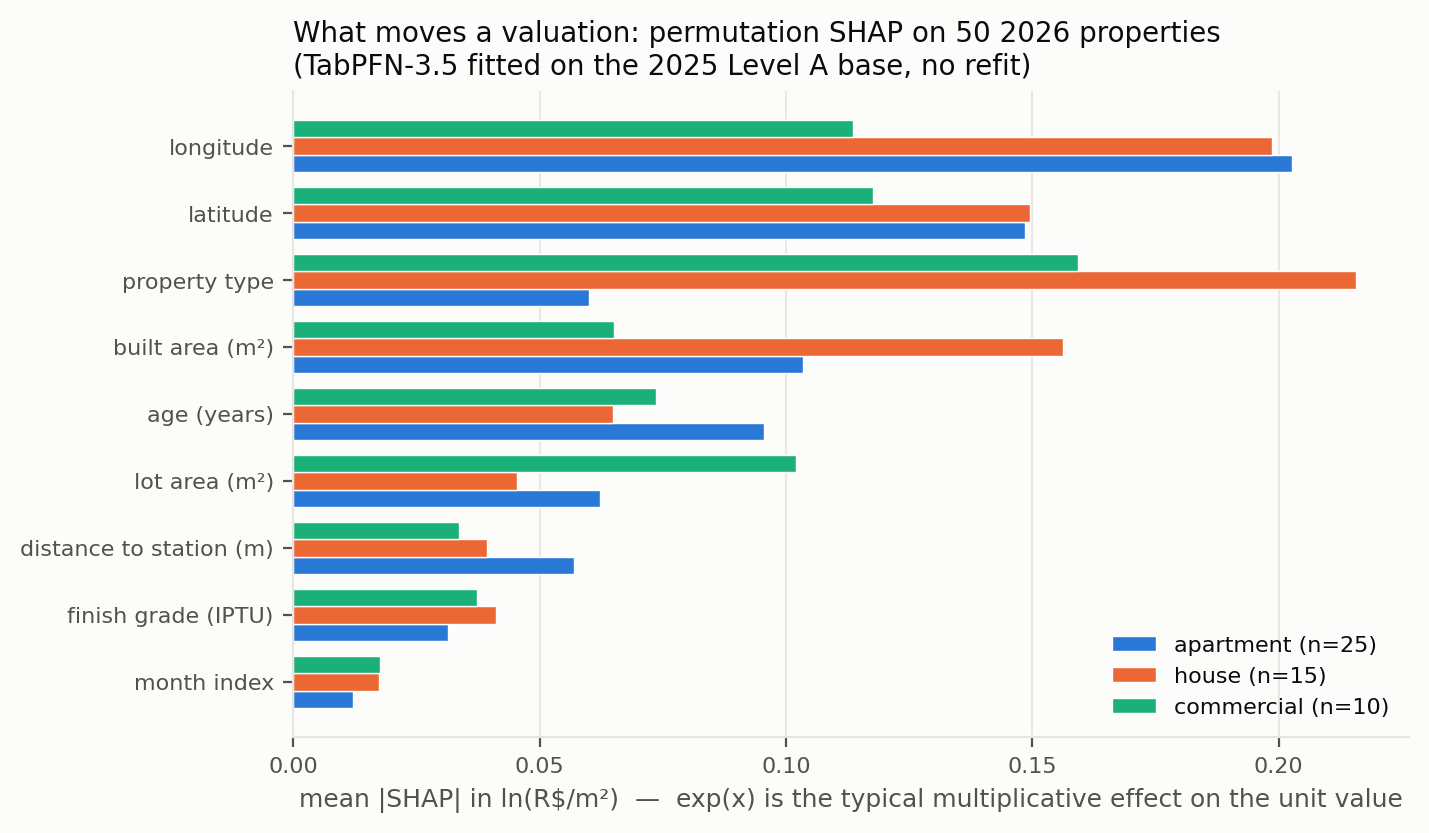
\includegraphics[width=\textwidth]{fig6_shap_importance.png}
\caption{Mean $|$SHAP$|$ by feature and type.}
\end{subfigure}\hfill
\begin{subfigure}[t]{0.49\textwidth}
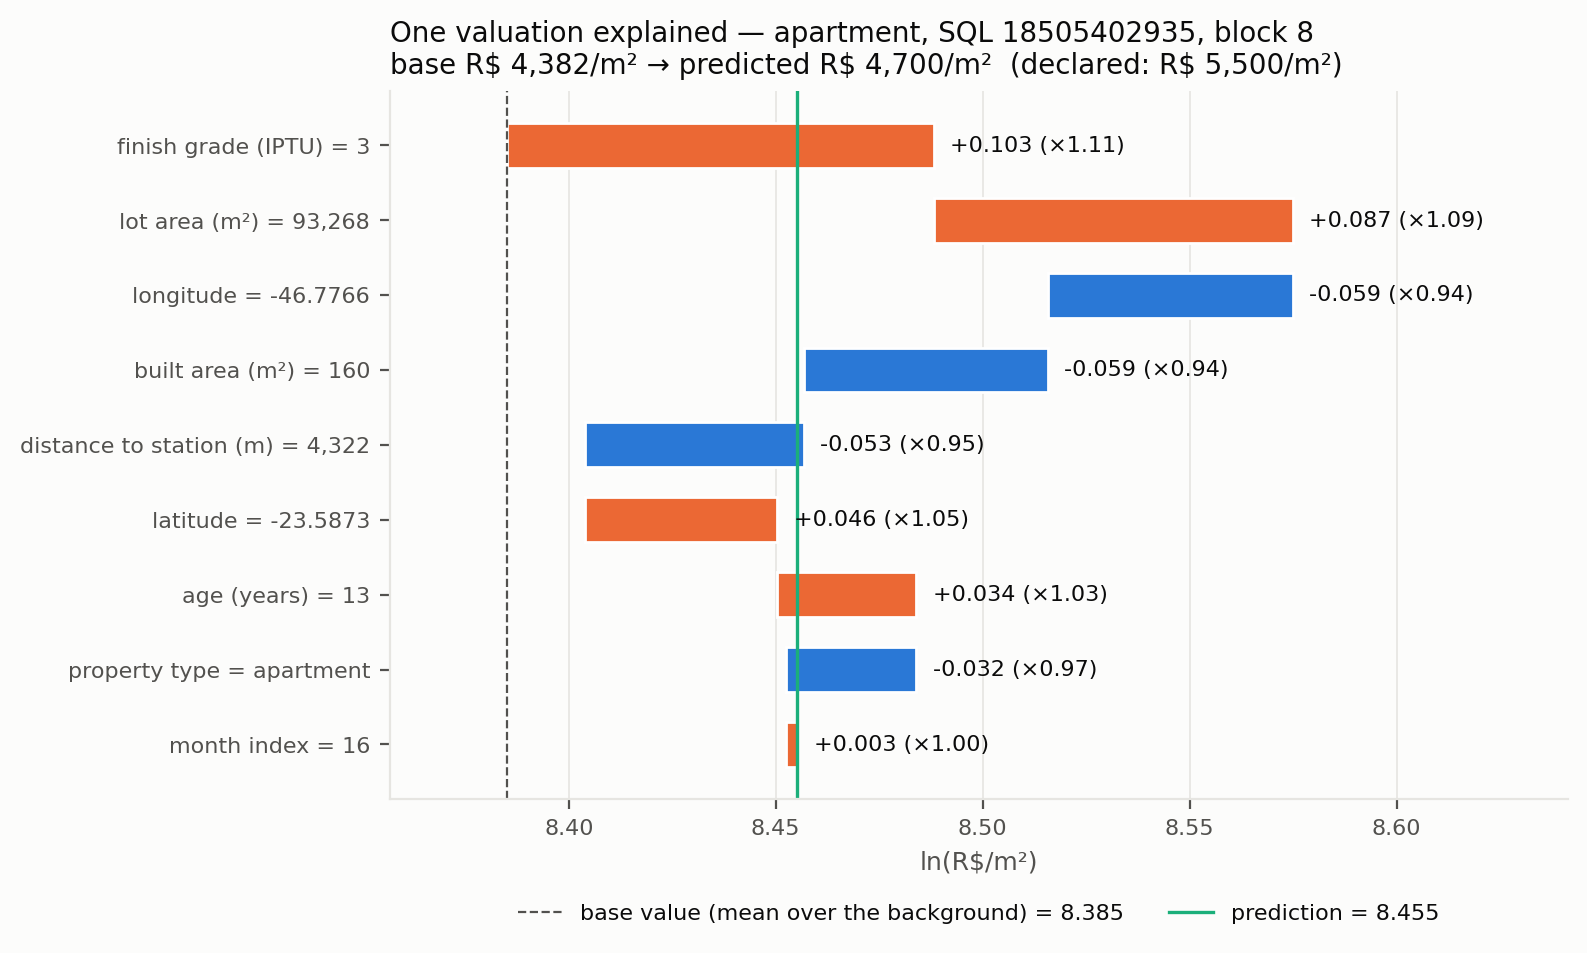
\includegraphics[width=\textwidth]{fig8_shap_waterfall.png}
\caption{One valuation, base value to estimate.}
\end{subfigure}
\caption{Permutation SHAP on 50 transactions of 2026 (independent masker, 20-row background),
model reloaded from its cached record. Values in log units; $e^{\text{SHAP}}$ is the multiplier
on the unit value.}
\label{fig:shap}
\end{figure}

An appraiser who signs a valuation has to say why. The model is served through an API, so the
explanation is model-agnostic permutation SHAP \citep{lundberg2017shap} on 50 stratified 2026
transactions the model had never seen, with every one of the 27{,}217 predicted rows cached for
offline reproduction. Reloaded from its cached record, the model reproduces the predictions it
is explaining (RMSE $0.296$ in ln on the 50 rows), so the attributions describe the run that was
scored. Longitude (mean $|$SHAP$|$ $0.184$, a typical $\times 1.20$ on the unit value) and
latitude ($0.143$, $\times 1.15$) are the two strongest inputs, ahead of property type
($0.127$), built area ($0.112$) and age ($0.082$). Directions match appraisal experience: age
and distance to a station pull the unit value down, finish grade pushes it up, larger built
areas lower the price per square metre. The two raw coordinates carry, inside the model, the
signal the baselines encode with a weights matrix --- and Section~\ref{sec:carriers} shows that
what they carry, within an observed market, is location as an identifier rather than geometry.

\section{Discussion}
\label{sec:discussion}

Read together, the two legs draw one line. Inside a market the model has seen --- the same city,
one to seven months ahead --- in-context learning over 24{,}000 to 82{,}000 rows recovers the
neighbourhood structure from two raw columns and prices better than the models built to encode
it, by every pre-registered criterion, residual autocorrelation included. The postal-code
variant sharpens the reading: within that market the model does not need geometry at all, only a
fine-grained location identifier, and it prices codes it has never seen among known ones almost
as well as known codes. Across the line, in a district with no sales in the training base, the
identifier collapses, the coordinates still extrapolate, and the explicit spatial lag earns its
keep on the residual criterion: the partial refutation of leg 1 is the measured price of not
modelling space when the test block is new ground. That price shrinks with more information ---
the free text of the form cuts the gap and the error --- and does not appear on the
lender-audited financed prices against XGBoost+lag; it does not vanish in the main analysis, and
it is reported as found.

The one systematic error shared by all models is the trend. Every model under-predicts the
rising market of 2026, the non-linear learners more ($+0.04$ to $+0.10$ in ln against $+0.02$ to
$+0.03$ for the linear models), because trees and the foundation model hold the last observed
level of the month index instead of extrapolating it. Appraisal practice corrects this with a
price index as a matter of routine; no correction was applied here, so that the comparison
stays between models as fitted. The bias concerns the level rather than location: the residual maps and
Moran's $I$, which the trend shifts uniformly, still separate the models.

The engineering ledger is short. The SAR model needs a weights matrix per fold; the spatial
XGBoost needs a fold-internal lag, rotated axes and 30 nested tuning trials (about 15 minutes of
tuning on the full base); the geographically weighted XGBoost needs 1{,}000 local models and an
inner search over bandwidth and blend (about ten minutes). TabPFN-3.5 needs the table: one fit
of 9 to 15 seconds, and, where a postal code is already on the form, not even a geocoder. For
mass appraisal under the Brazilian standard NBR 14653-2, two consequences follow. The
standard's precision grades are defined on interval estimates, and the model returns predictive
quantiles at no extra engineering --- they are cached for every zero-shot fit in this study, and
their coverage analysis is the natural next step. And the standard's demand that a valuation be
grounded can be met in part by model-agnostic attribution: the SHAP directions above are the
ones an appraiser would defend.

The limits of the evidence are these. Coordinates are fiscal-block centroids, so location is
resolved to the city block and all transactions of one block coincide; a sub-metre deterministic
jitter breaks ties for the weights matrices only. Prices are self-declared; the
under-declaration filter removes the detectable bunching, not the phenomenon, and the
financed-only robustness bounds its effect. The study covers one city and one period, and the
foundation model is served through an API: its internals are not inspectable (hence no exact
per-row attribution for the regression head), and the hosted version can change, though the
weights are published for research use and every API response is cached. The TabPFN input
variants ran on a single seed; the plain-table seed spread in leg 1 ($0.003$ in ln) is far below
every leg-2 margin, but the leg-1 ties should be read with that width in mind. The
geographically weighted XGBoost is an approximation of the published estimator --- local models
at 1{,}000 regression points rather than at every training row, shared local hyper-parameters,
a bandwidth floor of 50 neighbours that the inner search chose in 8 of 10 folds --- defensible
on geographically weighted regression's own terms, and bounded by the bandwidth sensitivity
reported above. The shuffled-code test that would settle why unseen postal codes work is
designed, not run.

\section{Conclusion}
\label{sec:conclusion}

The hypothesis was that a tabular foundation model receiving coordinates as two plain numeric
columns predicts spatially correlated prices as well as, or better than, models that encode
spatial dependence explicitly, and it was put at risk against three such specialists --- SAR,
XGBoost with a spatial lag and a geographically weighted XGBoost --- on 130{,}000 declared
transaction prices, with the refutation criteria written first. One year ahead, inside
the observed market, the hypothesis survives every criterion at both training scales: lower
pooled error than SAR, XGBoost with a spatial lag and a geographically weighted XGBoost, wins
in at least 9 of 10 spatial blocks against every seed of every opponent, and the least residual
spatial autocorrelation of the five models --- a verdict that stands even when the coordinates
are replaced by a raw postal code. In a district never seen, it ties the two XGBoost variants on
error, beats SAR, and is partly refuted on the residual criterion, leaving more spatial
structure than either XGBoost; the free text of the tax form narrows that gap and the
financed-only subset dissolves it against XGBoost+lag, but in the main analysis it stands. The
verdict could change elsewhere: another city or market, listings instead of declared prices, a
model version with row-level attribution for regression, or the shuffled-code test, are the
experiments that would move it. As it is, within a market that has a sales history,
none of the spatial machinery tested here improved on the raw table; its remaining value,
measured, is extrapolation to ground without sales.

\section*{Reproducibility and data availability}
Code, cleaned data, cached model responses and every number in this paper are at
\url{https://github.com/abenvenho/tabpfn-itbi-sp} (Apache-2.0); all source data is public
(municipal open data under the Brazilian access-to-information law). The pipeline was re-run
from a clean clone: the three bases were rebuilt byte-identical from the raw public workbooks,
and the smoke and baseline runs returned the documented numbers. Every number cited in this
manuscript is checked against the versioned results by \texttt{paper/check\_numbers.py}.

\section*{Acknowledgements}
This study was carried out as an entry to the Prior Labs TabPFN-3.5 Hackathon, whose
participant API credits funded the model runs.

\paragraph{AI-assistance statement.} The code of this study was developed with the assistance
of cloud AI tools --- Claude (Fable and Opus models) and ChatGPT (Astra) --- and of the locally
run models Qwen 3.8 Next Flash and Qwen 3 Coder Next. The cloud tools also assisted with
drafting, translation, literature search, figure generation and text revision. The experimental
design, the methodological decisions, the analysis of the results and the conclusions are the
author's, who reviewed and takes responsibility for the entire content.

\bibliographystyle{plainnat}
\bibliography{refs}

\appendix

\section{Geographically weighted XGBoost: feasibility pilot}
\label{app:gxgb}

The published implementation (\texttt{geoxgboost}) calibrates one local XGBoost, with its own
grid search, at every training row over a dense $n \times n$ distance matrix. A pilot on 200
rows with one bandwidth candidate took 18.7~s ($0.093$~s per spatial unit), which extrapolates
to about half an hour per bandwidth candidate per fold at the 19{,}117 training rows of a
Level A fold, about two days for ten candidates over ten folds, and 2.9~GB of distance matrix
per fold on the study machine (2 vCPU, 7~GB RAM;
\texttt{results/gxgb\_timing\_pilot.json}). The regression-point approximation of
Section~\ref{sec:methods} keeps the estimator --- local models, bi-square weights, blend with a
global model, nested bandwidth choice --- at about one minute per fit and ten per tuning.

\section{Hyper-parameters and model settings}
\label{app:hparams}

\paragraph{XGBoost + spatial features.} Nested Optuna, 30 TPE trials per outer fold, inner
leave-one-block-out on the training blocks, early stopping with up to 3{,}000 rounds. Search
space: learning rate $0.01$--$0.2$ (log), max depth $3$--$10$, min child weight $1$--$50$
(log), subsample $0.5$--$1$, colsample\_bytree $0.4$--$1$, $\lambda$ $10^{-3}$--$30$ (log),
$\alpha$ $10^{-3}$--$10$ (log), $\gamma$ $10^{-4}$--$1$ (log). Selected for the full-base
out-of-time fit (seed 42): learning rate $0.049$, depth $7$, min child weight $2.0$, subsample
$0.89$, colsample $0.56$, $\lambda$ $0.0033$, $\alpha$ $0.0041$, $\gamma$ $0.0031$, $398$
rounds; inner RMSE $0.351$; tuning time $901$~s
(\texttt{results/xgb\_params\_*.json}).

\paragraph{Geographically weighted XGBoost.} $M = 1{,}000$ regression points ($K$-means of the
training coordinates); local models with shared hyper-parameters ($300$ rounds, learning rate
$0.05$, depth $4$); global model with $800$ rounds, learning rate $0.05$, depth $6$; a query
predicted by the inverse-distance average of its $3$ nearest local models, blended by $\alpha$.
Bandwidth $k$ and $\alpha$ by nested inner block CV, grids in Section~\ref{sec:methods} (the
grid values scale with the training size, hence 40--176 on the 19--21k-row training folds of
Level A). Chosen: on Level A, $k$ per fold between 40 and 176 (leg 1) and $k = 50$ (leg 2); on
the full base, $k = 342$; $\alpha = 0.5$ throughout
(\texttt{results/gxgb\_params\_*.json}).

\paragraph{TabPFN-3.5.} Hosted model, \texttt{tabpfn-client} 0.6.0,
\texttt{create\_default\_for\_version("v3.5")}, regression head, zero-shot unless stated.
Thinking mode: \texttt{thinking\_effort} medium or high, \texttt{thinking\_metric = "rmse"},
timeout 2{,}400~s; the grouped variant passes the spatial block as \texttt{group\_col}. The
82{,}187-row fits set \texttt{ignore\_pretraining\_limits}. Predictive quantiles are requested and cached on every zero-shot fit. Every API response is cached under
\texttt{results/tabpfn\_cache/}, so the full protocol re-runs offline from the cached
predictions.

\end{document}
